\chapter{Implementacja części sprzętowej}

Diagram, opisujący zaimplementowaną architekturę sprzętową przedstawiono na 
rysunku \ref{hw::arch}.

\begin{figure}[h!]
    \centering
    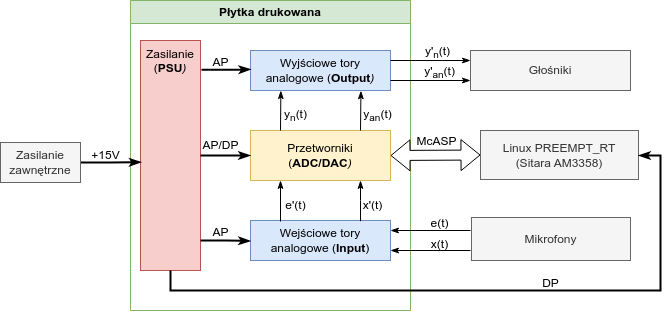
\includegraphics[width=\textwidth]{graf/hw/top.png}
    \caption{Architektura sprzętowa - najwyższy poziom}
    \label{hw::arch}
\end{figure}

Jak można zauważyć, na architekturę składają się cztery główne bloki:

\begin{enumerate}

    \item Zasilanie (\textbf{PSU}, ang. \textit{Power supply unit}) - sekcja 
    dopasowująca i propagująca zasilanie na cały układ. Prócz zasilań, które
    w przestrzenii projektowej nie są traktowane jak sygnały (są widoczne
    globalnie), łączy się z sekcją wejściowych torów analogowych poprzez
    wygenerowaną składową stałą (+1.25\_OFFSET).

    \item Wejściowe tory analogowe (\textbf{Input}, wejście)
    - sekcja przetwarzająca i dopasowująca sygnały dźwiękowe z mikrofonów pod 
    późniejszą konwersję do domeny cyfrowej. Łączy się z sekcją przetworników 
    poprzez przetworzone sygnały wejściowe (MIC\_IN, MIC\_ERR).

    \item Wyjściowe tory analogowe (\textbf{Output}, wyjście)
    - sekcja przetwarzająca i dopasowująca sygnały z przetworników 
    cyfrowo-analogowych pod dostarczenie do głośników. Łączy się z sekcją
    przetworników poprzez sygnały analogowe wypracowane przez przetworniki
    cyfrowo-analogowe (DAC\_OUT, DAC\_NOISE).

    \item Przetworniki (\textbf{ADC/DAC}) - sekcja opisująca połączenia 
    przetworników z interfejsem cyfrowym i resztą układu. Na jej wejście
    trafiają przetworzone sygnały z mikrofonów, a wychodzą sygnały z 
    przetworników cyfrowo-analogowych.

\end{enumerate}

\section{Urządzenia zewnętrzne}

\subsection{Mikrofony}

Przy wyborze mikrofonów do badań i testów implementacji kierowano się głównie
ceną i dostępnością. Nakierunkowane na pomiary modele czołowych marek są w 
zwyczaju relatywnie drogie, a jako, że w ramach pracy implementowane są dwa
kanały wejściowe, to kwestia ceny jest tutaj najbardziej decydującym wskaźnikiem.
\par Poza ceną i dostępnością, w omawianej tematyce uwagę należy zwrócić na
następujące parametry:

\begin{enumerate}

    \item Typ - standardem w omawianej tematyce są mikrofony \textbf{pojemnościowe}.
    Znane są z wysokiej czułości i płaskiej charakterystki częstotliwościowej, jednak
    wymagają dodatkowego zasilania, zwanego zasilaniem phantom.

    \item Charakterystyka kierunkowa - superkardoidalne lub hiperkardoidalne 
    mogą lepiej skupić się na kierunkowym źródle dźwięku, lecz w przypadku hałasu 
    w otwartej przestrzenii odbierany dźwięk będzie słabszy, jeżeli jego źródło 
    znajdzie się poza docelowym obszarem działania. Tematyka 
    projektu skupia się na hałasie w przestrzeni, a źródła dźwięku ustawione są
    względem siebie pod pewnym kątem, więc docelową charakterystyką jest 
    \textbf{charakterystyka kulista}.

    \item Odpowiedź częstotliwościowa - ideowo \textbf{płaska}. Zakres nie odgrywa
    znaczącej roli, bo analizowane sygnały są wolnozmienne (pasmo od 50 do 500 Hz, 
    gdzie typowe zakresy posiadają górną granicę definiowaną w dziesiątkach kiloherców).

    \item Czułość - informuje o wartości napięcia dla danego ciśnienia aktustycznego.
    Wynika z następującej zależności:
    \begin{equation} 
            S_{\text{dBV}} = 20 \text{log}_{10} \frac{S_{\text{mV/Pa}}}{U_{\text{ref}}}
    \end{equation}
    gdzie $U_{ref} = 1000 \text{ }\frac{\text{mV}}{\text{Pa}}$.  

\end{enumerate}

Na podstawie czułości mikrofonu dobiera się wzmocnienie przedwzmacniacza \cite{bib:mic}. 
Przykładowo, posiadając mikrofon z czułością na poziomie $10 \text{ }\frac{\text{mV}}{{\text{Pa}}}$,
uzyskuje się 10 mV dla 1 Pa, co jest równe 94 dB SPL.
Pracując na hałasach w zakresie 80 do 100 dB SPL, dla górnej granicy otrzymuje 
się 2 Pa, czyli odpowiednio 20 mV. W przypadku przetwornika analogowo-cyfrowego 
pracującego w przedziale -2.5 do 2.5 V, 20 mV z mikrofonu powinno odpowiadać maksymalnemu 
zakresowi 2.5 V, co pozwala na obliczenie wzmocnienia.

\begin{equation}
        k = \frac{U_{out}}{U_{mic}} = \frac{2.5}{0.02} = 125 \approx 42 \text{ dB} 
\end{equation}

Biorąc pod uwagę powyższe kwestie, autor zdecydował się na wykorzystanie 
mikrofonów Behringer ECM8000. Są one bardzo często wybierane przez amatorów
jak i profesjonalistów w zastosowaniach pomiarowych oraz cieszą się dobrymi 
opiniami. Ich droższym odpowiednikiem jest flagowy Beyerdynamic MM1, a najbardziej 
znaczące parametry są następujące \cite{bib:behringer}:

\begin{enumerate}

    \item Typ - pojemnościowy, phantom +15 do +48 V, akceptowalny przez sprzęt.

    \item Charakterystyka kierunkowa - kulista.

    \item Odpowiedź częstotliwościowa - relatywnie płaska, z
    pofalowaniami w paśmie 5 do 10 kHz i zakresie 20 do 20000 Hz.

    \item Czułość - $15 \text{ }\frac{\text{mV}}{{\text{Pa}}}$.

\end{enumerate}

\subsection{Zestaw głośnikowy}

Nie wchodząc w nadmierne i niepotrzebne w ramach pracy technikalia dotyczące 
typów i charakterystyk głośników, wybrane zestawy muszą spełnić trzy główne wymagania:

\begin{enumerate}

    \item Z racji, że zrezygnowano z projektowania końcówki mocy, wymagany 
    jest wbudowany wzmacniacz. Innymi słowy, zestawy muszą być \textbf{aktywne}.

    \item Analizowane sygnały są wolnozmienne (pasmo 100 do 500 Hz), więc 
    wymagane jest wsparcie dla tonów niskich. Innymi słowy na wyposażeniu zestawu
    musi być głośnik niskotonowy (ang. \textit{woofer}), zdolny do emisji
    sygnałów akustycznych o niskiej częstotliwości.

    \item Z uwagi na zakres poziomu akustycznego analizowanych sygnałów, 
    zestaw musi być zdolny do osiągnięcia jego górnego limitu, czyli użytecznego 
    90 dB SPL.

\end{enumerate}

Na użytek prywatny, autor posiada parę monitorów studyjnych 
KRK Classic 8, spełniających wszystkie powyższe wymagania. Nie wchodząc w 
techniczne szczegóły, z najbardziej znaczących parametrów można wyróżnić \cite{bib:krk}:

\begin{enumerate}

    \item Typ i konfiguracja - aktywny, głośnik wysoko i nisko tonowy (ang. \textit{woofer, tweeter}).

    \item Maksymalny zakres poziomu akustycznego - 103 dB SPL, 106 dB SPL w piku.

    \item Charakterystyka częstotliwościowa do $\pm 3$ dB - 42.5 do 35000 Hz, płaska.

    \item SNR - poniżej 100 dB.

\end{enumerate}

\section{Zasilanie}

Diagram dystrybucji zasilania przedstawiono na rysunku \ref{hw::power_dist}.

\begin{figure}[h!]
    \centering
    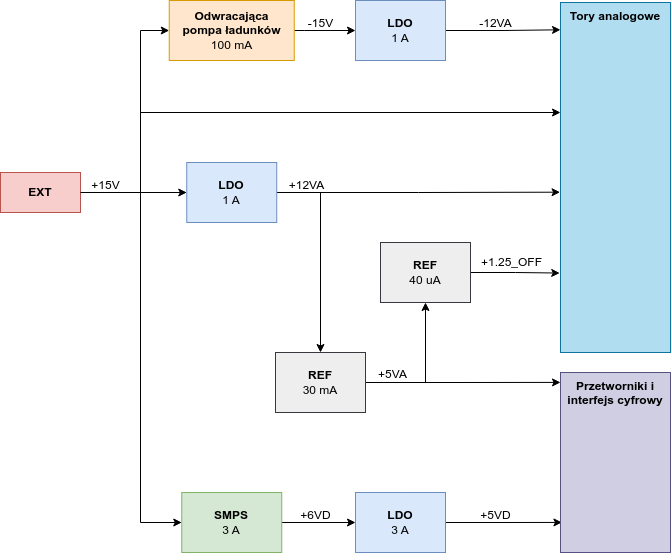
\includegraphics[width=\textwidth]{graf/hw/power_dist.png}
    \caption{Diagram dystrybucji zasilania}
    \label{hw::power_dist}
\end{figure}

\subsection{Sekcja wejściowa}

Układ zasilany jest z zewnętrznego zasilacza impulsowego o napięciu wyjściowym 
15 V. Zasilacze impulsowe znane są wysokiej, wynikającej z przełączania wewnętrznego
klucza tranzystorowego, fluktuacji napięcia wyjściowego (ang. \textit{ripple}), które w przypadku dobranego 
zasilacza wynosi maksymalnie 240 mV p-p.
Na uwadze należy również mieć zakłócenia pochodzące z sieci, wraz z przeregulowaniami powstającymi 
w momentach włączenia i wyłączenia układu.
\par Typowym rozwiązaniem stosowanym w sekcjach wejściowych układów elektronicznych
jest zastosowanie dolnoprzepustowego filtru LC, mającego za zadanie 
wygładzenie zewnętrznego zasilania jak i zapewnienie bufora do dalszych
konwersji. Taki filtr opisany jest następującą zależnością, wynikającą z uogólnionego 
równania dzielnika napięciowego \cite{bib:tietze}:
\begin{equation}
    U_{wy}(s) = U_{we}(s) \frac{Z_1}{Z_1 + Z_2} = U_{we}(s)\frac{\frac{1}{Cs}}{Ls + \frac{1}{Cs}}
        \implies K_{LP}(s) = \frac{1}{LCs^2 + 1}
    \label{eq:lc_lp}
\end{equation}
W dziedzinie symbolicznej natomiast ($s = j\omega$):
\begin{equation}
    K_{LP}(j\omega) = \frac{1}{1 - \omega^2LC}
\end{equation}

Częstotliwość rezonansowa takiego układu wynosi:
\begin{equation}
    \omega_c = 2\pi f_c \implies f_c = \frac{1}{2\pi\sqrt{LC}}
\end{equation}

Należy mieć na uwadze, że zależność \ref{eq:lc_lp} przedstawia idealny model układu LC.
W rzeczywistości każdy element pasywny posiada swoją rezystancję, przez co układ LC 
staje się układem RLC. Rezystor w takim układzie wprowadza tłumienie, z czego wynika
współczynnik tłumienia oraz dobroć. 
Wielkości te odpowiednio określone są następującymi zależnościami:
\begin{equation}
    \zeta = \frac{1}{2Q} = \frac{1}{2R\sqrt{\frac{C}{L}}}
    \label{eq:zeta}
\end{equation}
\begin{equation}
    Q = \frac{1}{R}\sqrt{\frac{L}{C}}
\end{equation}

Współczynnik tłumienia może znajdować się w czterech typach zakresów:
\begin{enumerate}
    \item $\zeta = 0$ - brak tłumienia, nieskończone oscylacje
    \item $\zeta > 0$ i $\zeta < 1$ - tłumienie subkrytyczne, oscylacje są wygaszane po pewnym czasie
    \item $\zeta = 1$ - tłumienie krytyczne, powrót do stanu ustalonego jak najszybciej i bez oscylacji
    \item $\zeta > 1$ - nadmierne tłumienie
\end{enumerate}


Przy projektowaniu tego typu układów oczekuje się, że będą tłumione krytycznie.
Oznacza to, że układ jest na granicy oscylacji, a pik rezonansowy na charakterystyce
częstotliwościowej jest nabliższy zakresowi pasma przenoszenia, 
które nie jest tłumione (możliwe płaskie) \cite{bib:lc}.
\\
\par W związku z tym, podstawiając $\zeta = 1$ w równaniu \ref{eq:zeta} otrzymuje się:
\begin{equation}
    L = \frac{R\sqrt{2}}{\omega_0}, \quad C = \frac{1}{\omega_0 R\sqrt{2}}
\end{equation}

Jako rezystancję przyjmuje się rezystancję wewnętrzną cewki.
W zaprojektowanym układzie $L = 4.7 \text{ }\mu$H i $C = 1080 \text{ }\mu$F,
z czego wynika $f_c \approx 2.47$ kHz oraz warunek na rezystancję cewki:
\begin{equation}
    R = \sqrt{\frac{L}{2C}} = \sqrt{\frac{4.7}{2160}} \approx 46.6 \text{ m}\Omega
\end{equation}
W układzie dobrano dostępną wartość najbliższą obliczeniom i wynosi ona $74.8 \text{ m}\Omega$. 
Warto wspomnieć, że w przypadku doboru rzeczywistych wartości elementów, w tym przypadku 
lepiej wybrać element o wartości zawyżonej niż zaniżonej, ponieważ bardziej oczekiwane
jest uzyskanie lepszego tłumienia, niż wzmocnienia pasma rezonansowego.
Omawiany schemat układu wraz z dołożonymi kondensatorami zapewniającymi dodatkowe
buforowanie i filtrację średnich częstotliwości przedstawiono na rysunku \ref{hw::input}:

\begin{figure}[h!]
    \centering
    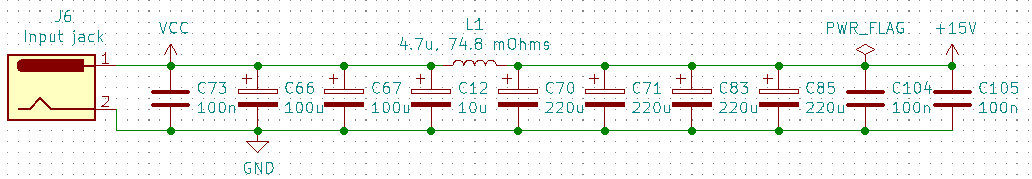
\includegraphics[width=\textwidth]{graf/hw/input.png}
    \caption{Sekcja wejściowa}
    \label{hw::input}
\end{figure}

\subsection{Symetryzacja szyn zasilających}

Przetwarzany sygnał dźwiękowy jest symetryczny wokół zera, więc wymagane jest,
również symetryczne zasilanie dla wzmacniaczy w sekcji torów analogowych, 
odpowiednio wysokie, aby nie doporowadzać do saturacji ich wyjść. 
Wybranym zasilaniem jest $\pm$12 V, a szczegóły dotyczące
tego wyboru będą dokładniej opisywane w sekcji torów analogowych.

\par Autor stosunkowo sporo czasu poświęcił kwesti generacji ujemnego zasilania.
W literaturze \cite{bib:art} \cite{bib:tietze} opisanych jest wiele sposobów implementacji tego typu 
układów, z czego najbardziej popularnymi są inwertery napięciowe zaimplementowane w oparciu o 
wzmacniacze operacyjne lub dedykowane przetwornice (ang. \textit{buck-boost}).

\par Rozwiązanie oparte o skonstruowanie układu inwerterów zostało odrzucone z 
powodu dodatkowego nakładu pracy. Taki system, poza układem 
odwracającym napięcie (ang. \textit{rail splitter}) wymagałby dodatkowego 
wzmacniacza mocy na wyjściu. Jest to spowodowane zapotrzebowaniem prądowym 
wzmacniaczy, które według specyfikacji wynosi maksymalnie 2.5 mA na układ. 
Jako, że w projekcie wykorzystywanych jest pięć wzmacniaczy operacyjnych na kanał, a 
kanałów jest cztery, to wymaganiem jest, aby wydajność prądowa wykorzystanego
generatora ujemnego napięcia wynosiła maksymalnie 100 mA. Opcja wyboru
dedykowanej przetwornicy została odrzuca z powodu niskiej dostępności układów 
zgodnych z założoną specyfikacją na rynku.

\par Wynikowo zdecydowano się na wykorzystanie układu 
odwracającej pompy ładunków. Układ spełnia wszystkie założenia projektowe i 
jest wydajny prądowo (maksymalny pobierany prąd równy 100 mA), minusem
jednak jest mała dokładność napięcia wyjściowego z dużymi fluktuacjami, 
opisanymi zależnością:
\begin{equation}
    U_{r,p-p} \approx \frac{I_{out}}{C_{out}}(\frac{1}{f_{osc}} - t_{on})
\end{equation}
W wykorzystywanym trybie pracy $t_{on} = 1 \text{ }\mu$s, $f_{osc} = 500$ kHz,
$I_{out} = 100$ mA i $C_{out} = 10 \text{ }\mu$ F, więc przewidywana aplituda
wyjściowych fluktuacji wyniesie 10 mV.

\par Dopuszczenie takiego napięcia na wzmacniacze w sekcji analogowej jest niedopuszczalne, 
między innymi zważając na wskaźnik PSRR, który dla wybranych wzmacniaczy wynosi
około 40 dB dla częstotliwości 500 kHz oraz niską dokładność.

\par W związku z powyższymi kwestiami, napięcie wyjściowe pompy ładunków należy
filtrować i stabilizować. Jako filtr zastosowano ponownie układ LC 
(rzeczywisty RLC) o niższej częstotliwości rezonansowej, ponieważ celem jest
filtracja fluktuacji wprowadzanych przez pompę ładunków. Dla dobranego 
$L = 3.3 \text{ }\mu$H i $C = 57 \text{ }\mu$F uzyskano $f_c \approx 12.18$ kHz 
oraz warunek na rezystancję cewki $R \approx 170 \text{ m}\Omega$, który 
spełniono wybierając najbliższą dostepną wartość równą 250 m$\Omega$.

\par Przefiltrowane ujemne napięcie trafia następnie wraz z jego dodatnim
odpowiednikim na układy liniowych regulatorów napięcia o małym spadku 
(LDO, ang. \textit{Low-dropout}), których celem jest stabilizacja oraz 
zwiększenie dokładności. Wykorzystane układy według specyfikacji dla zakresu 
pracy od 12 do 15 V posiadają dokładność równą 2.5\%, wydajność prądową równą 
maksymalnie 1 A oraz średni stosunek tłumienia zakłóceń równy 66 dB dla częstotliwości
powyżej 100 kHz i prądu wyjściowego równego 10 mA.

\par Omawiany układ wraz z dołożonymi kondensatorami odsprzęgającym, których
wartości dobierane były według not aplikacyjnych producenta przedstawiono na rysunku
\ref{hw::split}.

\begin{figure}[h!]
    \centering
    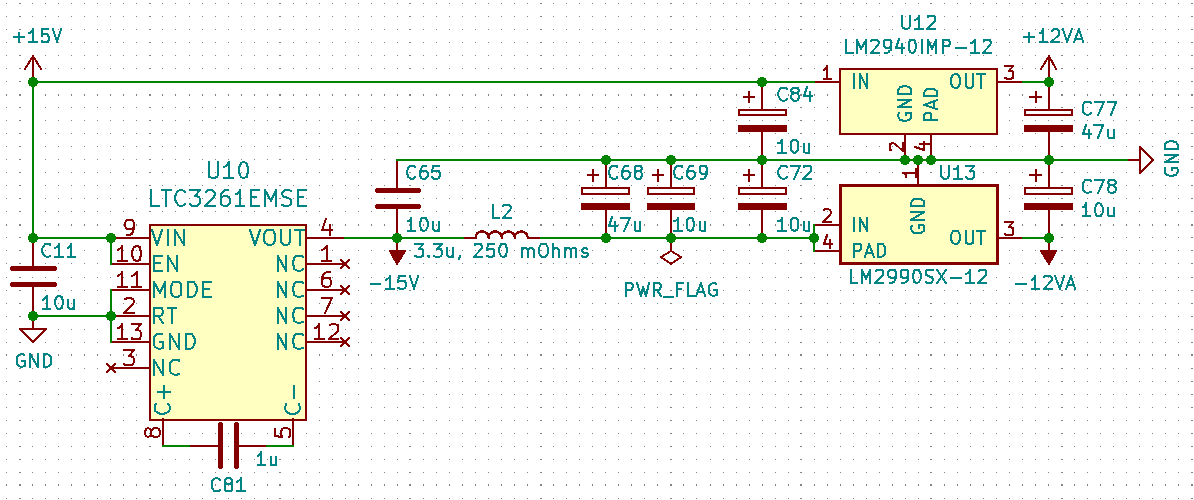
\includegraphics[width=\textwidth]{graf/hw/split.png}
    \caption{Symetryzacja szyn zasilających}
    \label{hw::split}
\end{figure}


\subsection{Zasilanie domeny cyfrowej}

Celem sekcji jest wygenerowanie napięcia równego 5 V, będącego zasilaniem
przetworników cyfrowo-analogowych oraz wybranej platformy rozwojowej.
Maksymalne zapotrzebowanie prądowe tych elementów wynosi odpowiednio 100 $\mu$A 
oraz około 2 A.
\par Wykorzystywana platformowa rozwojowa posiada własną sekcję stabilizacji i 
filtracji napięcia wejściowego, a wybrane przetworniki cyfrowe-analogowe, w przeciwieństwie 
do analogowo-cyfrowych, generują wyjście na podstawie dodatkowego sygnału 
referencyjnego, więc wymagania nałożone na dokładność wygenerowanego zasilania
są zdecydowanie mniej rygorystyczne niż w przypadku zasilań i referencji 
domeny analogowej.
\par Zważając na powyższe, w celu generacji napięcia wykorzystano układ 
impulsowej przetwornicy napięcia (\textbf{SMPS}, ang. \textit{Switched mode power supply}),
który jest tani, prosty w implementacji oraz zapewnia wysoką wydajność prądową, która
według dokumentacji wynosi do 3 A.
\par Zależność opisująca napięcie wyjściowe wykorzystanego układu podana jest 
przez producenta i zdefiniowana jest poniższym równaniem:
\begin{equation} 
    U_{out} = 0.765 \cdot (1 + \frac{R_1}{R_2})
    \label{eq::smps}
\end{equation}
Jak opisywano w sekcji dotyczącej filtracji i stabilizacji zasilania wejściowego,
przetwornice generują fluktuacje na wyjściu, które należy filtrować. W przypadku
tego układu, producent w nocie aplikacyjnej przedstawił zalecane parametry
wyjściowego filtru LC, z których skorzystano.
\par Napięcie z przetwornicy trafia końcowo na regulator napięcia w celu
stabilizacji oraz zostaje wyprowadzone na pozostałe sekcje. Omowiany układ
przedstawiono na rysunku \ref{hw::smps}.

\begin{figure}[h!]
    \centering
    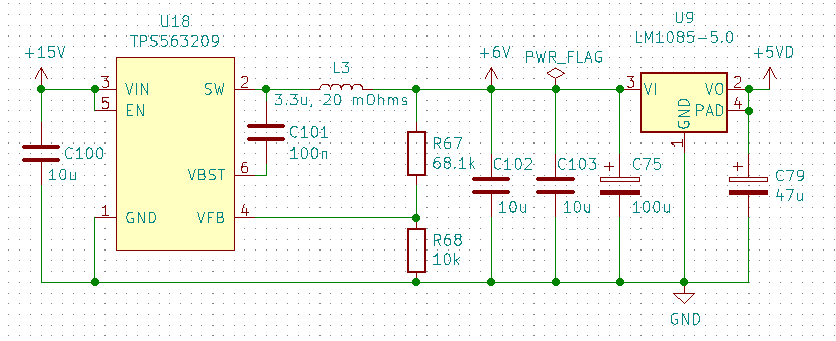
\includegraphics[width=\textwidth]{graf/hw/smps.png}
    \caption{Zasilanie domeny cyfrowej}
    \label{hw::smps}
\end{figure}

Napięcie wyjściowe przetwornicy zgodnie z zależnością \ref{eq::smps} wynosi
5.97 V, co pozwala poprawną stabilazację z wykorzystaniem regulatora 
niskiego spadku. Do wygenerowanego zasilania równolegle wraz z rezystorem
ograniczającym prąd dodatkowo podłączono diodę LED, działającą jako indykator
informujący o włączonym układzie.

\subsection{Referencja domeny analogowo-cyfrowej}

Wykorzystane przetworniki wymagają zasilania referencyjnego, na bazie 
którego przeprowadzane sa konwersje. W przypadku przetworników cyfrowo-analogowych,
zależność wynosi:
\begin{equation}
    U_{out} = \frac{U_{ref} \cdot D}{2^{N}}
\end{equation}
gdzie $D$ to dane załadowane do rejestru przetwornika, a $N$
to rozdzielczość. W przypadku przetwornika analogowo-cyfrowego, referencja wpływa
bezpośrednio na rozmiar kwantu:
\begin{equation}
    q = \frac{U_{ref}}{2^{N}}
\end{equation}

Z powyższych równań wynika, że sygnał referencyjny musi być bardzo dokładny.
Aby to uzyskać, zastosowano precyzyjny regulator napięcia niskiego spadku, zdolny
do generacji napięcia wyjściowego z maksymalnym błędem równym 2 mV i maksymalnym
obciążeniem równym 30 mA, wystarczającym dla wykorzystanych przetworników.
Zakres wejściowych napięć układu zawiera się w przedziale od -0.3 do +18 V,
więc wejściowe napięcie (równe +12 V) jest również odpowiednie. Omawiany
układ wraz z kondensatorami odsprzęgającymi przedstawiono na rysunku

\begin{figure}[h!]
    \centering
    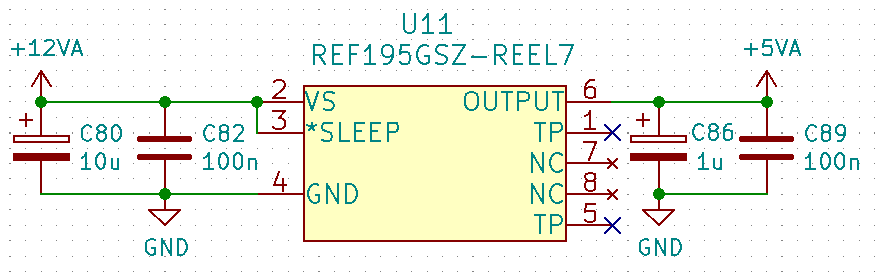
\includegraphics[width=\textwidth]{graf/hw/ref.png}
    \caption{Referencja domeny analogowo-cyfrowej}
    \label{hw::smps}
\end{figure}

Warto dodać, że napięcie referencje, prócz przetworników, trafia również na
ograniczniki diodowe zastosowane w sekcji wejściowych torów analogowych.

\subsection{Generacja składowej stałej}

Jak dokładniej będzie opisywane w sekcji torów analogowych, w celu zapewnienia 
pełnego zakresu dynamicznego przetworników analogowo-cyfrowych, niezbędny
jest dokładny i stabilny sygnał referencyjny zapewniający odpowiednią 
składową stałą w przetworzonym sygnale dźwiękowym trafiającym na wejście
przetwornika. Od układu generującego taki sygnał nie jest wymagana obsługa 
dużych obciążeń, ponieważ sygnał na jego wyjściu w zaimplementowanym
rozwiązaniu trafia na wejście nieodwracające wzmiacniaczy operacyjnych 
w sekcji analogowej, których impedancja wejściowa jest liczona w M$\Omega$ 
(teoretycznie impedancja wejściowa wzmacniacza operacyjnego jest nieskończona 
\cite{bib:art}).
\par W celu generacji takiego sygnału posłużono się układem napięcia odniesienia, 
który wraz z niezbędnymi kondensatorami odsprzęgającymi przedstawiono na rysunku
\ref{hw::off}.

\begin{figure}[h!]
    \centering
    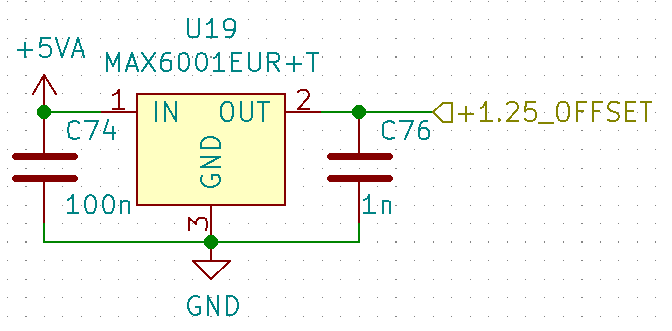
\includegraphics[width=\textwidth]{graf/hw/off.png}
    \caption{Układ napięcia odniesienia}
    \label{hw::off}
\end{figure}

\section{Wejściowe tory analogowe}
\subsection{Zasilanie Phantom}
\subsection{Wejściowa filtracja zakłóceń dużej częstotliwości}
\subsection{Wzmocnienie różnicowe}
\subsection{Filtracja antystroboskopowa}
\subsection{Pozycjonowanie}
\subsection{Zabezpieczenia}
\section{Wyjściowe tory analogwe}
\subsection{Kondycjonowanie wstępne}
\subsection{Wzmocnienie}
\subsection{Filtracja rekonstrukcyjna}
\subsection{Symetryzacja}
\subsection{Kondycjonowanie końcowe}
\section{Przetworniki}
\subsection{Analogowo-cyfrowe}
\subsection{Cyfrowo-analogowe}
\section{Protokół cyfrowy}
\subsection{Kondycjonowanie}
